\documentclass[11pt]{article}

\usepackage[margin=1in]{geometry}
\usepackage{amsmath,amssymb}
\usepackage{booktabs}
\usepackage{graphicx}
\usepackage{hyperref}
\usepackage{tikz}
\usetikzlibrary{arrows.meta, positioning}


% --- BIBLIOGRAFIA "CHE FUNZIONA" SU OVERLEAF ---
% Mettiamo le entry BibTeX direttamente dentro al .tex
\begin{filecontents*}{references.bib}
@article{fama1970efficient,
  title={Efficient Capital Markets: A Review of Theory and Empirical Work},
  author={Fama, Eugene F.},
  journal={The Journal of Finance},
  volume={25},
  number={2},
  pages={383--417},
  year={1970}
}

@article{barmish2015control,
  title={On the Control of Stock Trading Using Feedback},
  author={Barmish, B. Roy and Primbs, James A.},
  journal={IEEE Transactions on Automatic Control},
  volume={60},
  number={9},
  pages={2403--2410},
  year={2015}
}

@article{bollerslev1986generalized,
  title={Generalized Autoregressive Conditional Heteroskedasticity},
  author={Bollerslev, Tim},
  journal={Journal of Econometrics},
  volume={31},
  number={3},
  pages={307--327},
  year={1986}
}

@book{wilder1978new,
  title={New Concepts in Technical Trading Systems},
  author={Wilder, J. Welles},
  year={1978},
  publisher={Trend Research}
}

@article{jegadeesh1993returns,
  title={Returns to Buying Winners and Selling Losers: Implications for Stock Market Efficiency},
  author={Jegadeesh, Narasimhan and Titman, Sheridan},
  journal={The Journal of Finance},
  volume={48},
  number={1},
  pages={65--91},
  year={1993}
}

@article{lo2004adaptive,
  title={The Adaptive Markets Hypothesis},
  author={Lo, Andrew W.},
  journal={The Journal of Portfolio Management},
  volume={30},
  number={5},
  pages={15--29},
  year={2004}
}

@article{moreira2017volatility,
  title={Volatility-Managed Portfolios},
  author={Moreira, Alan and Muir, Tyler},
  journal={The Journal of Finance},
  volume={72},
  number={4},
  pages={1611--1644},
  year={2017}
}

@book{campbell1997econometrics,
  title={The Econometrics of Financial Markets},
  author={Campbell, John Y. and Lo, Andrew W. and MacKinlay, A. Craig},
  year={1997},
  publisher={Princeton University Press}
}
\end{filecontents*}

% Usa biblatex + biber (Overleaf lo gestisce bene)
\usepackage[backend=biber,style=apa]{biblatex}
\addbibresource{references.bib}

\title{Empirical Limits of Model-Free Feedback Trading Strategies\\
under Discrete-Time and Self-Financing Constraints}
\author{Nicola Brandolini}
\date{December 2025}

\begin{document}
\maketitle

\begin{abstract}
Model-free feedback trading strategies have attracted attention in control and finance due to their robustness properties and minimal modeling assumptions. In particular, Simultaneous Long-Short (SLS) strategies have theoretical guarantees under idealized continuous-time settings. This paper evaluates SLS strategies on real equity data in a discrete-time, self-financing framework and tests practical extensions (volatility scaling via GARCH, RSI filtering, and sector-level filtering). Results suggest that feedback-based strategies can reduce volatility and drawdowns but do not deliver consistent excess returns relative to Buy-and-Hold in this setting.
\end{abstract}

\section{Introduction}
Efficient market arguments imply that systematic excess returns are difficult to obtain without predictive structure \parencite{fama1970efficient}. This motivates strategies that do not forecast returns directly. Model-free feedback trading, developed in the intersection of control and finance, provides one such framework \parencite{barmish2015control}. However, the translation from continuous-time theory to discrete-time empirical trading can reveal limitations \parencite{lo2004adaptive}. We provide an empirical assessment of SLS strategies and simple extensions.

\section{Data}
We use daily adjusted close prices for 25 large-cap equities (five sectors) from 2015-05-04 to 2017-05-04. Log-returns are computed as:
\[
r_t = \ln\left(\frac{P_t}{P_{t-1}}\right).
\]

\section{Trading Framework}
At time $t$, the portfolio holds $q_t$ shares and cash $c_t$, with value:
\[
V_t = q_t P_t + c_t.
\]
Trading is discrete-time at daily closes. Short-selling is permitted, but the portfolio is constrained to remain self-financing and non-negative ($V_t\ge 0$). Trades that would violate feasibility are rescaled to the maximum admissible size.

\section{Benchmarks}
\textbf{Buy-and-Hold} invests all initial capital at $t=0$ and holds the position. \\
\textbf{Random trading} samples target positions from a symmetric distribution and applies the same self-financing constraint; this is a sanity-check baseline.

\section{SLS Strategy}
The discrete-time SLS update is:
\[
q_{t+1} = q_t + k\,(P_t - P_{t-1}),
\]
with feedback gain $k>0$ \parencite{barmish2015control}.

\section{Volatility Scaling (GARCH)}
Conditional volatility is estimated with a GARCH(1,1) model \parencite{bollerslev1986generalized}:
\[
\sigma_t^2 = \omega + \alpha \varepsilon_{t-1}^2 + \beta \sigma_{t-1}^2.
\]
The gain is scaled as:
\[
k_t = \frac{k}{\sigma_t},
\]
motivated by volatility-managed portfolio ideas \parencite{moreira2017volatility}.

\section{RSI Filtering}
We compute RSI using Wilder’s smoothing \parencite{wilder1978new} and use it as a modulation mechanism (risk gating), not as a return predictor. Momentum effects are well documented in the literature \parencite{jegadeesh1993returns}.

\section{Sector-Level Filtering}
To reduce idiosyncratic noise, we combine each asset’s return with the average return of its sector peers, consistent with documented co-movement in equity returns \parencite{campbell1997econometrics}.

\begin{figure}[h]
\centering
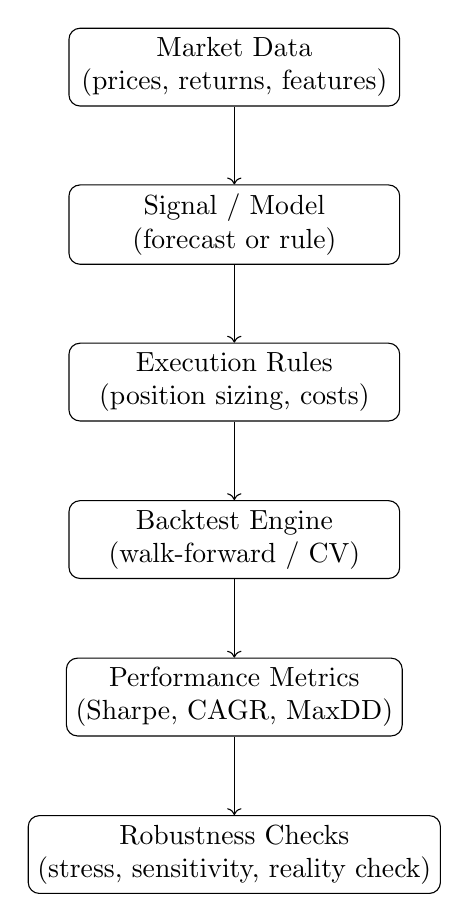
\begin{tikzpicture}[
  node distance=2.0cm,
  every node/.style={draw, rectangle, rounded corners, align=center, minimum width=4.2cm, minimum height=0.95cm}
]
\node (data) {Market Data\\(prices, returns, features)};
\node (signal) [below of=data] {Signal / Model\\(forecast or rule)};
\node (rules) [below of=signal] {Execution Rules\\(position sizing, costs)};
\node (bt) [below of=rules] {Backtest Engine\\(walk-forward / CV)};
\node (metrics) [below of=bt] {Performance Metrics\\(Sharpe, CAGR, MaxDD)};
\node (robust) [below of=metrics] {Robustness Checks\\(stress, sensitivity, reality check)};

\draw[->] (data) -- (signal);
\draw[->] (signal) -- (rules);
\draw[->] (rules) -- (bt);
\draw[->] (bt) -- (metrics);
\draw[->] (metrics) -- (robust);
\end{tikzpicture}
\caption{Experimental pipeline for strategy development and evaluation in algorithmic trading.}
\label{fig:trading_pipeline}
\end{figure}

\section{Results}
Across assets, SLS and extensions typically reduce volatility and drawdowns relative to Buy-and-Hold, but do not yield consistent positive excess returns in this discrete-time self-financing setting. Volatility scaling and filters improve stability but do not fundamentally change average excess performance.

\section{Discussion}
The findings highlight a gap between continuous-time theoretical guarantees and discrete-time empirical trading behavior. Feedback rules regulate exposure effectively but do not create predictive edge. Extensions based on volatility targeting and filters can improve risk characteristics without reliably generating excess return.

\section{Conclusion}
Under the tested assumptions and sample, model-free feedback trading is more effective as a risk-control mechanism than as a consistent alpha generator. Future work may explore hybrid schemes combining feedback control with predictive signals or different execution frequencies.

\printbibliography

\newpage


\appendix
\section{Algorithmic Implementation Details}

This appendix provides pseudo-code descriptions of the trading algorithms analyzed in the paper. The goal is to ensure full reproducibility of the experimental setup independently of any specific programming language.

\section{Self-Financing Trading Engine}

All strategies rely on a common self-financing execution engine.

\subsection*{Algorithm A1: Self-Financing Execution}

\begin{quote}
\textbf{Input:} Current price $P_t$, desired position $\tilde{q}_{t+1}$, current position $q_t$, current cash $c_t$ \\
\textbf{Output:} Updated position $q_{t+1}$, updated cash $c_{t+1}$
\end{quote}

\begin{enumerate}
\item Compute proposed trade:
\[
\Delta q = \tilde{q}_{t+1} - q_t
\]
\item Compute required cash:
\[
\Delta c = -\Delta q \cdot P_t
\]
\item If $c_t + \Delta c \ge 0$:
\begin{itemize}
\item Execute full trade: $q_{t+1} = \tilde{q}_{t+1}$, $c_{t+1} = c_t + \Delta c$
\end{itemize}
\item Else:
\begin{itemize}
\item Rescale $\Delta q$ so that $c_{t+1} = 0$
\item Set $q_{t+1} = q_t + \Delta q_{\max}$
\end{itemize}
\end{enumerate}

This mechanism ensures that the portfolio value remains non-negative at all times.

\section{Buy-and-Hold Strategy}

\subsection*{Algorithm A2: Buy-and-Hold}

\begin{quote}
\textbf{Input:} Initial capital $V_0$, initial price $P_0$
\end{quote}

\begin{enumerate}
\item Set $q_0 = V_0 / P_0$
\item Set $c_0 = 0$
\item Hold $q_t = q_0$ for all $t$
\end{enumerate}

\section{Random Trading Strategy}

\subsection*{Algorithm A3: Random Trading}

\begin{quote}
\textbf{Input:} Distribution $\mathcal{D}$ over target positions
\end{quote}

At each time step $t$:
\begin{enumerate}
\item Sample target position:
\[
\tilde{q}_{t+1} \sim \mathcal{D}
\]
\item Apply Algorithm A1 to enforce self-financing
\end{enumerate}

\section{Simultaneous Long-Short (SLS) Strategy}

\subsection*{Algorithm A4: Discrete-Time SLS}

\begin{quote}
\textbf{Input:} Feedback gain $k$
\end{quote}

At each time step $t$:
\begin{enumerate}
\item Observe price change:
\[
\Delta P_t = P_t - P_{t-1}
\]
\item Compute target position:
\[
\tilde{q}_{t+1} = q_t + k \cdot \Delta P_t
\]
\item Apply Algorithm A1
\end{enumerate}

\section{Volatility-Scaled SLS}

\subsection*{Algorithm A5: GARCH-Scaled SLS}

\begin{quote}
\textbf{Input:} Base gain $k$, GARCH volatility estimate $\sigma_t$
\end{quote}

At each time step $t$:
\begin{enumerate}
\item Compute scaled gain:
\[
k_t = \frac{k}{\sigma_t}
\]
\item Compute target position:
\[
\tilde{q}_{t+1} = q_t + k_t \cdot \Delta P_t
\]
\item Apply Algorithm A1
\end{enumerate}

\section{RSI Filtering}

\subsection*{Algorithm A6: RSI Computation (Wilder Smoothing)}

\begin{quote}
\textbf{Input:} Period $n$, price series $\{P_t\}$
\end{quote}

\begin{enumerate}
\item Initialize average gain and loss over first $n$ observations
\item For $t > n$:
\[
\text{avg\_gain}_t = \frac{(n-1)\,\text{avg\_gain}_{t-1} + \max(P_t - P_{t-1}, 0)}{n}
\]
\[
\text{avg\_loss}_t = \frac{(n-1)\,\text{avg\_loss}_{t-1} + \max(P_{t-1} - P_t, 0)}{n}
\]
\item Compute:
\[
RS_t = \frac{\text{avg\_gain}_t}{\text{avg\_loss}_t}, \quad
RSI_t = 100 - \frac{100}{1 + RS_t}
\]
\end{enumerate}

\subsection*{Algorithm A7: RSI-Filtered SLS}

At each time step $t$:
\begin{enumerate}
\item Compute $RSI_t$
\item Define modulation factor $m_t \in [0,1]$ based on RSI thresholds
\item Update position:
\[
\tilde{q}_{t+1} = q_t + m_t \cdot k \cdot \Delta P_t
\]
\item Apply Algorithm A1
\end{enumerate}

\section{Sector-Level Complementary Filter}

\subsection*{Algorithm A8: Sector-Filtered Signal}

\begin{quote}
\textbf{Input:} Asset return $r_t^{(i)}$, sector peer returns $\{r_t^{(j)}\}_{j \neq i}$
\end{quote}

\begin{enumerate}
\item Compute sector average:
\[
\bar{r}_t^{(-i)} = \frac{1}{N-1} \sum_{j \neq i} r_t^{(j)}
\]
\item Construct filtered signal:
\[
\hat{r}_t^{(i)} = \lambda r_t^{(i)} + (1-\lambda)\bar{r}_t^{(-i)}
\]
\item Use $\hat{r}_t^{(i)}$ in place of $\Delta P_t$ in Algorithm A4
\end{enumerate}

\section{Summary of Algorithmic Structure}

All strategies can be viewed as instances of the following generic update:
\[
\tilde{q}_{t+1} = q_t + g_t \cdot s_t,
\]
where $s_t$ is a signal derived from observed prices and $g_t$ is a possibly time-varying gain. The self-financing constraint (Algorithm A1) enforces feasibility and ensures comparability across strategies.

\section{Statistical Evaluation and Robustness}

This appendix describes the statistical metrics and aggregation procedures used to evaluate strategy performance.

\subsection{Return and Risk Metrics}

For each asset and strategy, the following quantities are computed over the full sample horizon:

\begin{itemize}
\item \textbf{Cumulative return}:
\[
R = \frac{V_T - V_0}{V_0}
\]

\item \textbf{Annualized volatility}:
\[
\sigma_{\text{ann}} = \sqrt{252}\,\mathrm{std}(r_t)
\]

\item \textbf{Maximum drawdown (MDD)}:
\[
\text{MDD} = \max_{t \le s} \left( \frac{V_s - V_t}{V_s} \right)
\]

\item \textbf{Sharpe ratio (uncorrected)}:
\[
\text{Sharpe} = \frac{\mathbb{E}[r_t]}{\mathrm{std}(r_t)} \sqrt{252}
\]
\end{itemize}

No risk-free rate adjustment is applied, as the analysis focuses on relative comparisons across strategies.

\subsection{Excess Performance}

Performance is primarily evaluated through excess return relative to the Buy-and-Hold benchmark:
\[
\alpha = R_{\text{strategy}} - R_{\text{BH}}.
\]

This quantity measures incremental performance attributable to active trading rather than market exposure.

\subsection{Cross-Sectional Aggregation}

Results are aggregated across the cross-section of assets using simple averages:
\[
\bar{\alpha} = \frac{1}{N} \sum_{i=1}^{N} \alpha^{(i)}.
\]

The distribution of $\alpha^{(i)}$ across assets is also analyzed to assess heterogeneity and robustness.

\subsection{Bootstrap Confidence Intervals}

To assess statistical uncertainty without relying on parametric assumptions, block bootstrap resampling is employed. Daily returns are resampled in contiguous blocks of fixed length $L$ to preserve serial dependence.

For each bootstrap sample $b = 1, \dots, B$:
\begin{enumerate}
\item A resampled return series is constructed.
\item Strategy performance metrics are recomputed.
\item The empirical distribution of $\alpha^{(b)}$ is obtained.
\end{enumerate}

Confidence intervals are computed as percentile intervals of the bootstrap distribution. This procedure is used exclusively for robustness assessment and not for formal hypothesis testing.

\subsection{Multiple Testing Considerations}

Given the evaluation of multiple assets and parameter configurations, no formal hypothesis testing is conducted at the individual asset level. Reported results emphasize consistency of qualitative behavior rather than statistical significance of isolated outcomes.

This conservative approach reduces the risk of spurious findings due to multiple comparisons.

\section{Replication Statement}

This study is fully reproducible using publicly available data and open-source software.

\subsection{Data Availability}

All price data used in this study consist of daily adjusted closing prices obtained from Yahoo Finance. The complete list of assets and the sample period are specified in Section~2. No proprietary datasets are used.

\subsection{Code Availability}

The complete source code used to generate all results in this paper, including data preprocessing, strategy implementation, and performance evaluation, is available upon request and will be released in a public repository upon publication.

The code is written in Python and relies exclusively on widely used open-source libraries.

\subsection{Computational Environment}

All experiments were conducted using a standard desktop computing environment. No specialized hardware or proprietary software is required. Randomized components of the experiments (e.g., random trading strategies and bootstrap procedures) are controlled via fixed random seeds to ensure reproducibility.

\subsection{Reproducibility Notes}

All trading strategies are implemented under explicitly stated assumptions regarding self-financing constraints and execution timing. No look-ahead bias or future information is used in signal construction.

Minor numerical discrepancies may arise across computing environments due to floating-point arithmetic, but these do not affect the qualitative conclusions of the study.

\end{document}